\chapter{SaaS, le tecnologie che ne consentono la realizzazione}

\section{SaaS e i suoi requisiti}

\subsection{Availability}
Il concetto di Availability, nel senso generale del termine, è ben definito dallo standard ITU-T E.800: "L'abilità di un sistema di essere in uno stato che soddisfa un determinato requisito, in determinati istanti di tempo, assumendo che le risorse a lui necessarie siano disponibili." Come possiamo vedere, è un concetto ben definito, ad ha quindi le sue metriche ben definite che quantificano l'Availability. 

\paragraph{MTTF, Mean Time TO Failure}
Misura l'intervallo di tempo tra due eventi di "faiulure", in cui il sistema non è riuscito a portare a termine il proprio compito.

\paragraph{}
Possiamo dire quindi che l'Availability rappresenta la porzione di tempo in cui il sistema si comporta secondo le proprie specifiche. Va tenuto in considerazione anche che, al verificarsi di un fallimento, al tempo di non-Availability si aggiunge il tempo per porre rimedio al fallimento e far ripartire il sistema. 

\paragraph{}
Possiamo immaginare, a questo punto, quanto sia fondamentale un'altissima availability per i servizi Cloud 


la figura va al capitolo dopo
\begin{figure}[h!]
	\centering
	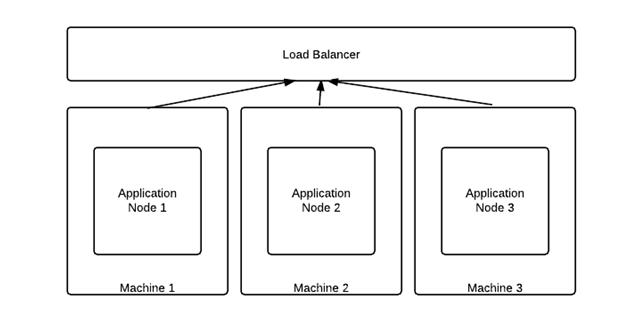
\includegraphics[width=\textwidth,keepaspectratio=true]{capitoli/imgs/LoadBalancer.png}
	\caption{Una schematizzazione della distribuzione del carico in una architettura Cloud}
\end{figure}
